\section{Phase space, Hamiltonian dynamics, and the fundamental postulate of statistical mechanics}
\subsection{Phase space}

\begin{figure}[h]
    \centering
    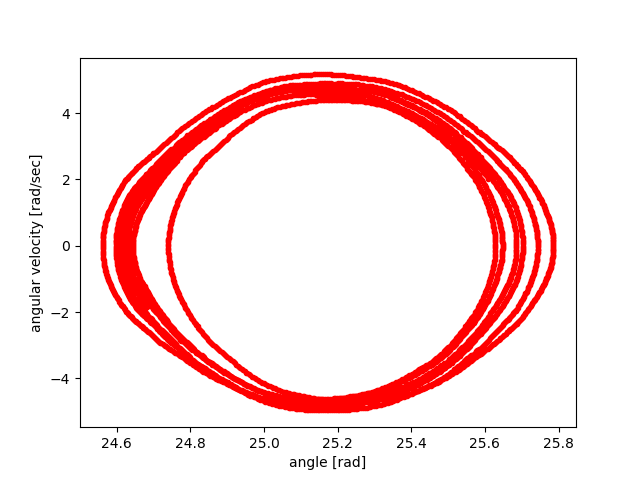
\includegraphics{chaotic_pendulum_stable}
    \caption{Phase space for a chaotic (damped, driven) pendulum in a stable oscillation}
    \label{fig:chaotic_pendulum}
\end{figure}

At a microscopic level, a thermodynamic system is comprised of $N$ particles, each with some mass $m_i$, which can interact with each other and with the boundaries of the system. (Although we are going to motivate this discussion with a thermodynamic system, everything the follows is also true for other systems where the total energy of the system is conserved --- i.e. anywhere that a Hamiltonian could show up.) If we know the positions and momenta  for each of the particles then we can completely describe the state of the system. In three dimensions, this means we must know the values for each of the $6N$ degrees of freedom (3 for position and 3 for momentum); more generally, we have $2d$ d.o.f. where $d$ is the number of d.o.f. for the positions. That is the state of the system is described by a point in a $6N$ (or $2d$) dimensional \textit{phase space}.

\begin{definition}[Phase Space]
We call a $6N$-dimensional space the phase space of a given system, if each degree of freedom of the system corresponds to exactly one axis of the space.
\end{definition}

Once a point in the microscopic phase space is known, the evolution of the system is completely governed by the equations of motion for the system. These in turn are prescribed by the Hamiltonian of the system

\begin{equation}
    H = T+U = H({\bf r}, {\bf v}) = H({\bf q}, {\bf p})
\end{equation}
where $T=$ kinetic energy, $U=$ potential energy. In general, $H$, $T$, and $U$ may all depend on both the positions and the momenta of the particles, however, for many systems we find that, conveniently, $T = \sum_{i=1}^{N} T_i$, where $T_i=\frac{{\bf p}_i^2}{2m_i}$, and the potential $U$ depends only on the positions: $U = U({\bf q}).$

If the Hamiltonian is known for a system, then the equations of motion for that system are given by the \textit{Hamiltonian equations of motion}:
\begin{eqnarray*}
	\frac{d{\bf q}_i}{dt} &=& ~~\frac{\partial H}{\partial {\bf p_i}}, \\
	\frac{d{\bf p}_i}{dt} &=& -\frac{\partial H}{\partial {\bf q_i}}.
\end{eqnarray*}

If we write ${\bf x} = [{\bf q}^\top,{\bf p}^\top]^\top$, then we can compactly express the equations of motion as

\begin{equation}
	\frac{d{\bf x}}{dt} = f({\bf x}) = J^{-1}\nabla H({\bf x}),
\end{equation}
where
$$
	J = 
	\begin{bmatrix}
		0 & -\mathbb{I}_d\\
		\mathbb{I}_d & 0
	\end{bmatrix}.
$$
($\mathbb{I}_d$ is the identity matrix of dimension $d$.)

Given a Hamiltonian, H, and a suitable set of initial conditions ${\bf x}_0$, the evolution of the solution ${\bf x}(t)$ can be quite complicated (Hamiltonian systems are one of the archetypal systems for studying chaotic dynamics). However, the fact that the system is Hamiltonian provides us with some additional information that can help us characterise the state of the system. For example, it is not hard to prove that a solution ${\bf x}(t)$ that satisfies $\dot{\bf x} = f({\bf x}) = J^{-1}\nabla H({\bf x}),$ ${\bf x}_0 = {\bf x}(0)$ has $H({\bf x}(t)) = H({\bf x}_0)= \text{const}.$ That is, Hamiltonian systems conserve energy along their solutions. We identify the Hamiltonian $H$ with the internal energy of the system.

Knowing that $\frac{dH}{dt}=0$, we can reduce the size of the phase space where ${\bf x}(t)$ can lie, from $2d$ d.o.f. down to $2d-1$. If we know other quantities that remain invariant over time (e.g. the total momentum of the system) then we can further reduce the size of the phase space. Strictly speaking, there are $2d-1$ invariants (AKA first integrals or constants of motion) for a Hamiltonian system. This defines a curve in the remaining 1 d.o.f. along which the solution must lie (that is, a line in the phase space). This can be seen as a consequence of the uniqueness theorem for differential equations (think back to the 2nd year maths course on D.E.s). In reality, we typically can't find a closed form expression for most of these conserved quantities and have no idea what they might be.

It is possible that a (vanishingly) small change in the positions of the particles in phase space can lead to a large change in the state of the system and in the subsequent trajectories of the particles\footnote{In Fig.~\vref{fig:chaotic_pendulum}, the chaotic pendulum was configured to be in a stable orbit, hence its well-behaved orbit in phase space}.
This is similar to saying that the dynamics of a Hamiltonian system can switch abruptly from regular to chaotic motion, as some parameter of the system is varied. Such quantities are not helpful in characterising the thermodynamics of the system. In statistical mechanics, we are interested in the invariant quantities that only change by a little when there is a small change in the microscopic variables of the system, i.e., ${\bf x}\rightarrow {\bf x}+\delta {\bf x} \implies H\rightarrow H+\delta H$.

One way to phrase this is to say that we want to consider systems where the region in phase space where the system is evolving can be (almost) completely identified, for thermodynamic purposes, by the values of a (not too large) number of observable invariant quantities.

\subsection{Observables}
In statistical mechanics, we say that an observable is a function defined on the phase space of the system that varies smoothly with changes in the representative point of the system. This definition is different to the definition in quantum mechanics.

The kinetic energy $\sum_i \frac{p_i}{2m_i}$ is an observable, while the function $\Theta = \prod_i \theta(r_0^2-r_i^2)$, where $\theta(x)$ is the Heaviside function, is not, since an arbitrarily small change in a position $r_i$ can lead to a finite change in $\Theta$. This behaviour is not smooth which means $\Theta$ is not an observable. This non-smoothness results from the presence of the Heaviside function (also known as the unit step function), which is equal to zero when its argument is negative and one when it is positive; this function has a jump when the argument is zero and is thus obviously not smooth.

Other examples of (thermodynamic) observables include the internal energy $E$ (i.e. the Hamiltonian) and the number of particles in the system ($N = \int d{\bf r}\sum\delta({\bf r}-{\bf r}_i)$).
It turns out that the entropy $S=S(X_0=E=H,X_1,\ldots,X_r)$ is also an observable. However, we don't yet have a way to express the entropy --- the extensive variable of a thermodynamic system --- as a function of the microscopic state of the system and its equations of motion. To do so, we are going to invoke the fundamental postulate of statistical mechanics.

\subsection{The fundamental postulate of statistical mechanics}
The fundamental postulate expresses the entropy $S$ as a function of the accessible volume of the phase space of a dynamical system. I.e. that part of the phase space where the observables have values that are compatible with a specific thermodynamic state.

Assume that the thermodynamic state of a system is determined by the extensive variables $X_1,\ldots,X_r$ and that each of the $X_i$ can be expressed as a function over the microscopic phase space; I.e. $X_i = X_i({\bf x})$.
The region of phase space that is accessible is defined by the value of $X = (X_1,\ldots,X_r)$. Well, almost; we actually also allow for small discrepancies $\epsilon_i,~~i=1,\ldots,r$ to account for the effect of any non-extensive terms.

We denote the region of phase space in which the observable $X_i$ have the specific values that match the thermodynamic state as $\Gamma$ and we denote the corresponding phase space volume $\text{vol}(\Gamma)=\Omega$. Then the fundamental postulate of thermodynamics states that
\begin{equation}
	S = k_B\ln(\Omega),
	\label{eqS}
\end{equation}
where $S$ is the thermodynamic entropy, $k_B$ is Boltzmann's constant ($k_B = 1.384\times10^{-23}$J/K) and the equality should be interpreted as meaning ``is equal, up to terms of size $\epsilon_i$''. The accessible phase space volume $\Omega$ measures the amount of the phase space available to the microscopic system while it is in this macroscopic state. If the system had only discrete micro-states, then we could simply count the number of micro-states that correspond to the same macro-state. 


\subsection{Symplectic transformations and phase space area preservation}
Why is phase space so important in the formulation of entropy? To understand this we are going to look closer at some of the properties that being Hamiltonian impose on a system, including the choice of coordinate system.

We saw earlier that the equations of motion for a time-independent Hamiltonian system can be written as $\frac{d{\bf x}}{dt} = f({\bf x}) = J^{-1}\nabla H({\bf x})$. This Hamiltonian form is not preserved by arbitrary coordinate transformations; it \emph{is} preserved by \emph{symplectic} transformations.

\begin{definition}
A linear transformation $A: \mathbb{R}^{2d}\rightarrow\mathbb{R}^{2d}$ is said to be symplectic if it satisfies
$$ A^\top J A = J.$$
\end{definition}

For a non-linear transformation $\mathcal{A}$, we replace $A$ above with its Jacobian $D\mathcal{A}$.

An alternative, but equivalent, definition of a symplectic transformation --- and one that will turn out to be useful in a bit --- borrows some tools from differential geometry. (No prior experience with differential geometry is assumed.)

\begin{definition}
A symplectic transformation is a diffeomorphism (a smooth, invertible mapping between manifolds) $f:\mathbb{R}^{2d}\rightarrow\mathbb{R}^{2d}$, with coordinates $q$ and $p$, which preserves the symplectic two-form $\omega$ (an anti-symmetric, bilinear form) that acts on pairs of vectors and gives the sum of the oriented areas that they define. In two dimensions, this is the area of the parallelogram spanned by the two vectors.

More explicitly,
\begin{equation*}
	\omega(u,v) = u^\top Jv = \sum_{i=1}^d u_{p_i} v_{q_i} - u_{q_i} v_{p_i}.
\end{equation*}
\end{definition}

At this point it is necessary to introduce a (potentially) new concept --- the flow map of a vector field. The flow $\varphi_{t,f}({\bf x})$ of a Hamiltonian system is a function that maps a point ${\bf x}^*$ in the phase space of the system with equations of motion $\dot{\bf x} = f({\bf x}) =J^{-1}\nabla H({\bf x})$ forward by time $t$. I.e. for any $f({\bf x})$ and ${\bf x}_0$, $\varphi_{t,f}({\bf x}_0)$ gives the solution to $\dot{\bf x}=f({\bf x})$ at time $t$. That is, it shows the time evolution of {\bf x} and {\bf p} on the phase space.\\

\begin{theorem}
If the Hamiltonian $H({\bf x})$ is a twice differentiable function on some neighbourhood of $\mathbb{R}^{2d}$, then the time-$t$ flow map $\varphi_{t,f}({\bf x}_0)$ of the Hamiltonian vector field is a symplectic map for all $t$.
\end{theorem}

\begin{proof}
We will show that $\omega(u,v)=u^\top J v$ is constant along solutions of $\dot{\bf x} = J^{-1}\nabla H({\bf x})$.

The tangent vector $u(t) = \frac{\partial \varphi_t}{\partial {\bf x}_0}({\bf x}_0)u(0)$ satisfies $\frac{du}{dt} = J^{-1}\nabla^2H({\bf x}(t))u(t)$ and the tangent vector $v(t)$ satisfies a similar expression. Now we can calculate the time derivative of $\omega(u,v)$.
\begin{eqnarray*}
	\frac{d}{dt}\omega(u,v) &=& \dot{u}^{\top}Jv+u^\top J\dot{v}\\
		&=& (J^{-1}\nabla^2Hu)^\top Jv + u^\top JJ^{-1}\nabla^2Hv\\
		&=& 0
\end{eqnarray*}
since $J^{-\top}=(J^{-1})^\top$, $J^{-\top}J=-I$ and $JJ^{-1} = I$.

i.e., as the system evolves according to its equations of motion, it always preserves the area for $d=1$, or the sum of the oriented areas for $d \geq2$.
\end{proof}


\subsection{Liouville's theorem and preservation of phase space volume}
We are now in a position to prove that the flow of a Hamiltonian system preserves phase space volume.

But first, why do we care about preservation of phase space volume? The fundamental postulate of statistical mechanics, $S=k_B\ln(\Omega)$ related the entropy of a system to the volume of the part of the phase space accessible to that system when it is in that particular thermodynamic state. We would like to be sure that this quantity doesn't vary too much over time as the microscopic system evolves, according to the Hamiltonian equations of motion. Although the microscopic system might be in continuous motion, the trajectories of the particles it is comprised of are such that the extensive variables which characterise the macroscopic state of the system are (almost) constant. I.e. there is no change in entropy, no heat flow, no work done while the system is at equilibrium. This is reassuring --- it says that disorder doesn't increase unless something happens.

\begin{theorem}[Liouville]
For every bounded, open set $A\subset\mathcal{R}^{2d}$ and every $t$ for which $\varphi_{t,f}({\bf x})$ exists
$$\text{Vol}(\varphi_{t,f}(\Gamma))=\text{Vol}(\Gamma)$$
where $f=J^{-1}\nabla H$ and $\text{Vol}(\Gamma) = \int_{\Gamma}d{\bf x}$
\end{theorem}

\begin{proof}
To prove this, we will actually prove a slightly more general case: the flow of a differential equation $\dot{\bf x}=f({\bf x})$ in $\mathbb{R}^n$ is volume preserving if and only if it is divergence-free; i.e. $\nabla\cdot f=0$.

The Jacobian of the flow map $\varphi_{t,f}({\bf x}_0)$ defines the matrix function $X(t)=D\varphi_{t,f}({\bf x}_0)$. The volume of the shape spanned by the columns of $X$ is given by $\det(X)$, and $X(t)$ is a solution of the equation
$$
\dot{X}=A(t)X(t),\qquad X(0)=I,
$$
where $A(t):=Df({\bf x}(t))$ denotes the Jacobian of $f({\bf x}(t))$ evaluated at ${\bf x}(t)=\varphi_{t,f}({\bf x}_0)$. To show that the volume defined by $X$ is constant we use the Abel-Liouville-Jacobi-Ostrogradskii identity to find the time derivative of $\det X$:
$$
\frac{d}{dt}\det X(t)=\text{trace} A(t)\cdot\det X(t).
$$
Since $A(t)=Df({\bf x}(t))$ we have $\text{trace} A(t)=\sum_i\frac{\partial f_i}{\partial {\bf x}_i}({\bf x}(t))=\nabla\cdot f({\bf x}(t))$ and therefore $\det X(t)=\det X(0)=1$ if and only if $\nabla\cdot f({\bf x})=0.$
\end{proof}

\subsection{Recommended reading}
This section has mostly followed the first half of chapter 3 of \emph{Statistical Mechanics in a Nutshell}. However, some of the significance of Hamiltonian systems is lost in SMiaN, so I've supplemented it with more substantive (mathematically oriented) details from \emph{Geometric Numerical Integration} by E. Hairer, Ch. Lubich and G. Wanner (Springer, 2006) --- one of the best books on (the numerics of) Hamiltonian dynamical systems and a personal favourite.
